\documentclass[a4paper,11pt]{article}

\usepackage[left=2cm,text={17cm, 24cm}, top=3cm]{geometry}
\usepackage[czech]{babel}
\usepackage[utf8]{inputenc}
\usepackage{times}
\usepackage{graphicx}
\usepackage{wrapfig}
\usepackage{floatrow}
\usepackage{siunitx}
\sisetup{output-decimal-marker = {,}}
\begin{document}
\begin{titlepage}
\begin{center}
\Huge
\textsc{Vysoké učení technické v~Brně\\ \huge Fakulta informačních technologií}\\
\vspace{\stretch{0.382}}
\Huge Fyzikální optika \\ 
\LARGE Hubbleův a Webbův teleskop - popis optických systémů  \\
\vspace{\stretch{0.109}}
semestrální projekt \\
\vspace{\stretch{0.309}}
\today
\vspace{\stretch{0.209}}
\end{center}
\Large Zdeněk Biberle - xbiber00@stud.fit.vutbr.cz \\ Josef Řídký - xridky00@stud.fit.vutbr.cz
\end{titlepage}
\newpage

\Large\noindent{\bf Abstrakt}\\
\normalsize\noindent\\ Tento projekt popisuje historii, vlastnosti a~popis optických soustav již používaného Hubbleova teleskopu a~plánovaného teleskopu Jamese Webba. V~první části je čtenář seznámen s~Hubbleovým teleskopem a~v~druhé části s~teleskopem Jamese Webba. Součástí tohoto projektu je i~animace popisující optické soustavy obou vesmírných teleskopů.\\
\vspace{\stretch{0.8}}\\
\Large\noindent {\bf Klíčová slova}\\
\normalsize\noindent teleskop, optické systémy, zrcadla, vesmír, Hubble, James Webb, NASA\\
\vspace{\stretch{0.2}}
\newpage

\tableofcontents

\newpage


\section{Úvod}
Člověk už od pradávna vzhlížel ke hvězdám a~vesmírným tělesům ve snaze je zdokumentovat, zaznamenat jejich pohyb či zajistit si jejich příznivé naklonění. V~posledních letech se však lidstvu díky technologickému pokroku podařilo udělat obrovský skok vpřed v~pozorování a~dokumentování naší galaxie a~vesmíru kolem nás. Díky rozmachu vesmírných programů se podařilo umístit přímo do kosmu speciální dužice a~teleskopy díky nimž jsme opět o~krok blíž k poznání tajů vesmíru. V~tomto semestrálním projektu se zabýváme historií, vlastnostmi a~popisem optických soustav dvou vesmírných teleskopů. Prvním teleskopem je Hubbleův teleskop, který je na oběžné dráze v~provozu již 25 let a~pomohl nám objasnit a~objevit mnoho záhad vesmíru. Druhým popsaným teleskopem je teleskop Jamese Webba, který ještě ve vesmíru není, avšak již existuje jeho model ve skutečné velikosti. Konstrukce finálního teleskopu je již v~plném proudu, aby mohl v~roce 2018 započít svoji misi. 

\section{Hubbleův vesmírný dalekohled}
Hubbleův vesmírný teleskop (známý také pod svou zkratkou HST, či pouze jako Hubble) je teleskop, který byl vypuštěn na oběžnou dráhu v roce 1990 \cite{nasaHubbleChronology}. Od té doby byly k teleskopu vyslány čtyři servisní mise \cite{hubbleSiteServicingMissions}, které postupně prodlužovaly až do původně očekávaného ukončení činnosti v roce 2015, NASA nyní ovšem tvrdí, že HST by mohl vydržet v provozu do roku 2018 \cite{hubbleUntil2018}, tedy do vypuštění vesmírného teleskopu Jamese Webba.

Díky HST jsme během jeho dvaceti pěti let provozu získali množství informací, které nám umožnily, mimo jiné, přesněji určit stáří vesmíru, pochopit procesy vedoucí k formování planet a rozšířit naše znalosti ohledně černých děr. Tyto informace také vedly k~objevu temné enrgie a~dokonce i~první organické molekuly mimo povrch Země \cite{nasaHubbleAccomplishments}.

\subsection{Historie}

Návrh na konstrukci vesmírného teleskopu vznesl poprvé v roce 1946 ve svém článku \cite{LymanSpitzer1990131}. Jako hlavní výhodu tohoto přístupu uvedl zbaevní se optických efektů Zemské atmosféry, které dosud limitovaly pozorování provedená pozemskými teleskopy.

Následně NASA v roce 1971 utvořila Large Space Telescope Science Steering Group, jejímž cílem bylo studium proveditelnosti vesmírného teleskopu o průměru tři metry. K tomuto projektu byla později v roce 1975 přizvána i European Space Agency. Průměr teleskopu byl zároveň zmenšen na 2,4 metry. 

V roce 1977 byl dokončen původní návrh teleskopu a~NASA přenechává práci na optickém systému společnosti Perkin-Elmer Corporation a~práci na pouzdru společnosti Lockheed Missiles and Space.


\begin{figure}[h]
	\begin{center}
		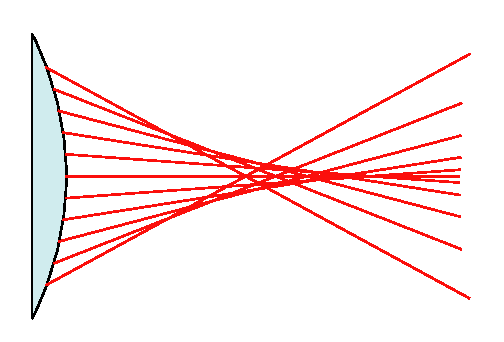
\includegraphics[width=6cm]{Spherical_aberration_2.eps}
		\caption{Vizualizace sférické aberace, kterou trpí primární zrcadlo HST.}
		\label{Spherical_aberration_2}
	\end{center}
\end{figure}

Práce na optickém systému a pouzdru byly dokončeny v letech 1984 a 1985.


Teleskop byl 24. dubna roku 1990 vynešen na oběžnou dráhu. Nedlouho poté je objevena, že hlavní zrcadlo teleskopu se vyznačuje sférickou aberací, což mělo za následek rozmazané snímky \cite{nasaHubbleChronology}.


\subsubsection{Servisní mise}
V roce 1993 byla k teleskopu vyslána první servisní mise STS-61, jejímž cílem bylo nainstalovat dvě nová zařízení - Wide Field and Planetary Camera 2 (WFPC2), tedy nový CCD optický senzor nahrazující původní WFPC, a Corrective Optics Space Telescope Axial Replacement (COSTAR), tedy korektivní optika, která měla omezit vliv sférické aberace hlavního zrcadla. Mise byla úspěšná a rapidně zvýšila ostrost snímků z HTS.

\begin{figure}[!h]
	\begin{floatrow}
		\ffigbox{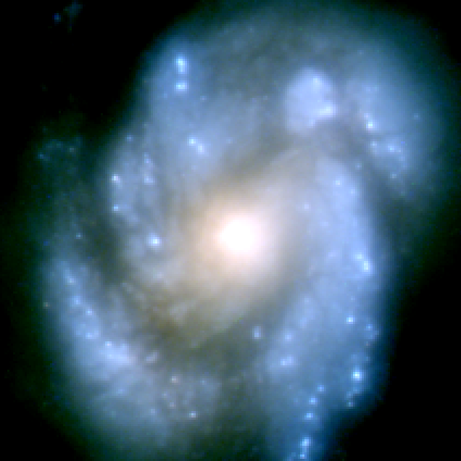
\includegraphics[scale = 0.6]{hubble-pre-wfpc2.png}}{\caption{Galaxie Messier 100 zachycená HST před instalací WFPC2 a COSTAR}\label{hubble-pre-wfpc2}}
		\ffigbox{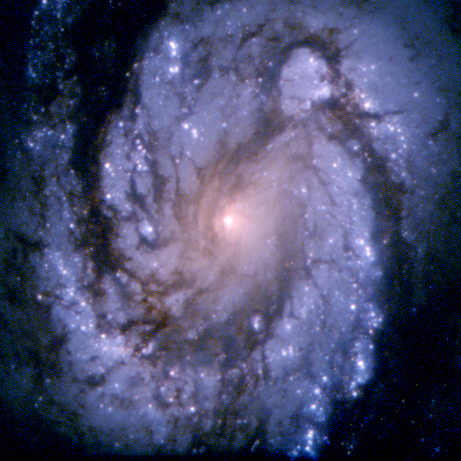
\includegraphics[scale = 0.6]{hubble-post-wfpc2.png}}{\caption{Galaxie Messier 100 zachycená HST po instalací WFPC2 a COSTAR}\label{hubble-post-wfpc2}}
	\end{floatrow}
\end{figure}

Druhá servisní mise (STS-82) byla provedena v roce 1997. Během této mise bylo nainstalováno několik dodatečných zařízení, primárně Near Infrared Camera and Multi-Object Spectrometer (NICMOS) a Space Telescope Imaging Spectrograph (STIS).

Třetí servisní mise byla rozdělena na dvě části. První části (STS-103) se uskutečnila ke konci roku 1999. Tato část byla zaměřena převážně na opravné a vylepšující práce. Druhá část (STS-109), uskutečněná v roce 2002, již měla větší efekt. Během této části došlo k instalaci Advanced Camera for Surveys (ACS), nové efektivnější solární panely, nový chladící systém pro NICMOS.

\begin{figure}[h]
	\begin{center}
		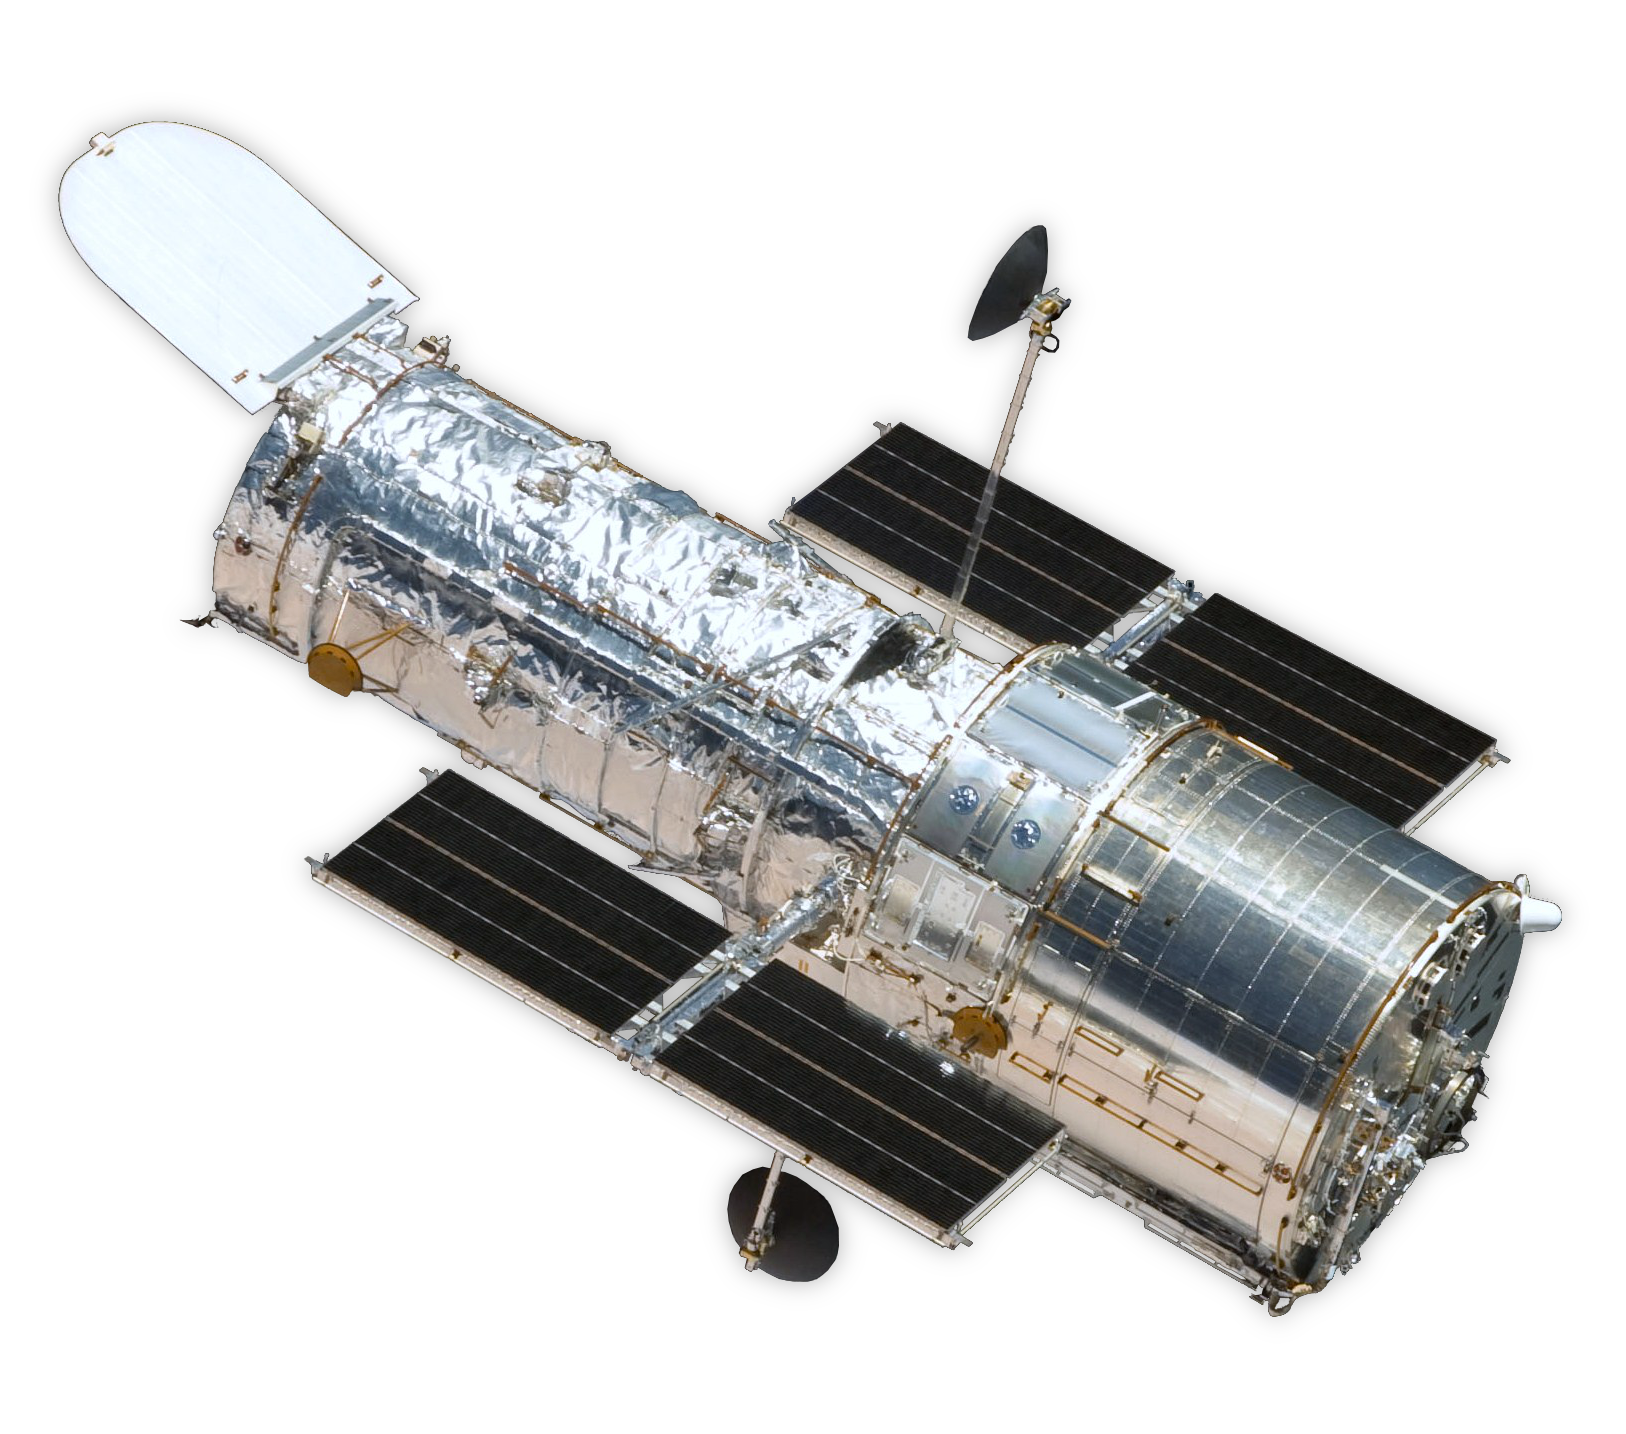
\includegraphics[width=8cm]{HST-SM4.png}
		\caption{Fotografie HST pořízená během STS-125}
		\label{HST-SM4}
	\end{center}
\end{figure}

Poslední, čtvrtá, servisní mise (STS-125) proběhla v roce 2009. Během této mise byl odstraněn modul WFPC2 a byl nahrazen novým modulem WFC3, tedy Wide Field Camera 3. Dále došlo k instalaci Cosmic Origins Spectrograph (COS). Zároveň byla odstraněna korektivní optika COSTAR, jelikož všechny systémy nainstalované na HST již byly konstruovány s vestavěnou korekcí. Zároveň došlo k opravě modulů ACS a STIS, které v letech 2007, resp. 2004, přestaly pracovat.

\subsection{Popis konstrukce}

HST je přibližně válcové konstrukce, o průměru až 4,2 m a délce a o délce 13,2 m. Po stranách HST se nachází dva solární panely dlouhé 7,6 m. Celý teleskop váží přibližně 11 tun. HST je tedy podstatně menší, ale zároveň lehčí, než jeho de facto nástupce, tj. Vesmírný teleskop Jamese Webba.

HST se v současnosti nachází na oběžné dráze 552 km nad Zemí a Zemi oběhne za 97 minut \cite{hubblesiteFacts}. HST není vybaven žádnými raketovými motory a pro orientaci jsou použita rotující kola.

\begin{figure}[h]
	\begin{center}
		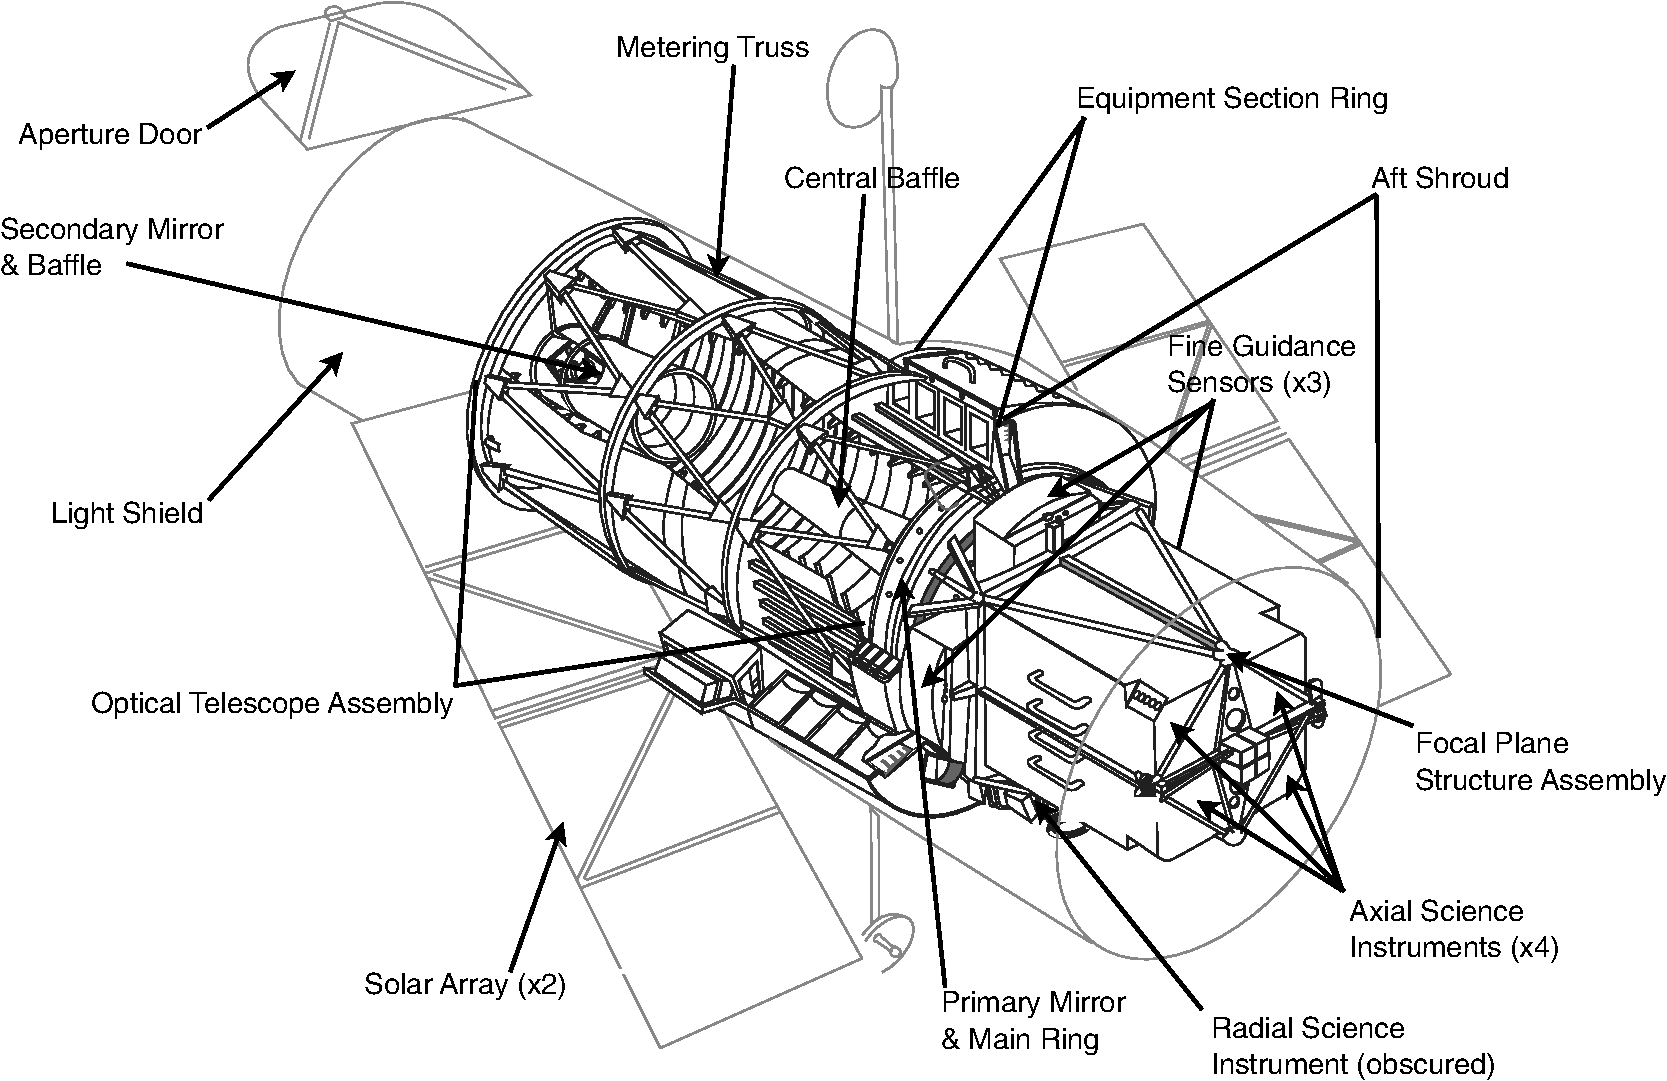
\includegraphics[width=16cm]{hst-structure.png}
		\caption{Struktura HST}
		\label{hst-structure}
	\end{center}
\end{figure}

Přední část HST je tvořena jednoduchým válcem, který částečně zabraňuje vstupu nežádoucího světla do teleskopu. Ke stejnému účelu slouží i žebrování uvnitř objektivu.

Za světelným štítem je umístěno sekundární zrcadlo. Poté následuje tzv. forward shell, tedy další kus žebrovaného objektivu. Za tímto se nachází Support Systems Module Equipment Section (SSMES), což je prstenec obsahující baterie, elektroniku, počítače, komunikační vybavení a manévrovací motory a kola. Ve středu tohoto prstence taktéž najdeme primární zrcadlo teleskopu.

Za primárním zrcadlem už se nachází snímací zařízení. Tato jsou rozdělena do dvou kategorií:
\begin{itemize}
	\item Radiální - Wide Field Camera 3 a Fine Guidance Sensors
	\item Axiální - Cosmic Origins Spectrograph, Advanced Camera for Surveys, Space Telescope Imaging Spectrograph a Near Infrared Camera and Multi-Object Spectrometer.
\end{itemize}

Snímací nástroje a SSMES jsou umístěny ve válcovém hliníkovém obalu. Zbytek teleskopu je obalen do Multi-Layered Insulation, tedy vícevrstvé izolace tvořené z teflonu pokrytého hliníkem.

\subsection{Vybavení}
Již víme, že na HST se nachází hned několik zařízení pro snímání přicházejícího světla. Tato zařízení jsou následující:
\subsubsection{Wide Field Camera 3}
WFC3 je kamera nacházející se v radiální sekci teleskopu, kde nahradila v roce 2009 předchozí Wide Field and Planetary Camera 2.

WFC3 pracuje v rozsahu od blízkého ultrafialového záření až po blízké infračervené záření.

Pro snímání ultrafialového a viditelného světelného záření je použit CCD senzor o rozlišení $4000 \times 4000$ pixelů. Pro Infračervené záření je pak použit senzor o rozlišení $1000 \times 1000$ pixelů \cite{ballWfc3}.

\subsubsection{Fine Guidace Sensors}
FGS jsou tři kamery umístěné taktéž v radiální sekci teleskopu, které jsou určené pro zaměřování teleskopu.

Dvě tyto kamery se typicky zaměří na dvě kotevní hvězdy a na základě jejich pozice a ve spolupráci s manévrovacími motory poté udržují teleskop v pozici zaměřené na cíl \cite{hubblesiteFgs}.

\subsubsection{Cosmic Origins Spectrograph}
COS se nachází v axiální části teleskopu od roku 2009, kdy nahradil korektivní optiku COSTAR. Jak již jeho název napovídá, tak se jedná o spektrograf. Konkrétně se jedná o spektrograf pracující v rozsahu ultrafialového záření \cite{hubblesiteCos}.

\subsubsection{Advanced Camera for Surveys}
ACS je druhé zařízení nacházející se v axiální části teleskopu. Jedná se o kombinaci tří zařízení \cite{stsciDetectors}:
\begin{itemize}
	\item Wide Field Channel - Kamera pro pořizování rozsáhlých snímků galaxie. Obsahuje dva CCD snímače o rozlišení $2048 \times 4096$ pixelů.
	\item High Resolution Channel - Kamera pro pořizování méně rozsáhlých snímků galaxie. Zasahuje více do ultrafialového záření, než WFC. Obsahuje jeden CCD snímač s rozlišením $1024 \times 1024$.
	\item Solar Blind Channel - Tato kamera má podobné vlastnosti jako HRC, ovšem snímá primárně ultrafialové záření.
\end{itemize}

\subsubsection{Space Telescope Imaging Spectrograph}
Opět zařízení umístěné v axiální části teleskopu. Podobně jako v případě COS se jedná o spektrograf, ovšem pracující i v rozsahu viditelného a blízkého infračerveného světla. STIS navíc funguje i jako běžná kamera. Zařízení obsahuje tři senzory (jeden CCD a dva MAMA), každý s rozlišením $1024 \times 1024$ a různým frekvenčním rozsahem \cite{stsciStisDetectors}\cite{hubblesiteStis}.

\subsubsection{Near Infrared Camera and Multi-Object Spectrometer}

NICMOS je finální zařízení nacházející se v axiální části teleskopu. NICMOS je infračervená kamera pracující v rozsahu \SI{0,8}{\um} až \SI{2,5}{\um}. Zařízení obsahuje tři detektory s rozlišením $256 \times 256$ pixelů, každý s aktivním chlazením \cite{stsciNicmosDetectors}\cite{stsciNicmosPerformance}.

\subsection{Optický systém}

Pohled na hlavní strukturu strukturu optického systému HST vidíme na obrázku \ref{hubble-structure}. Konstrukce je poměrně klasická, se zaostřením na nekonečno.

\begin{figure}[h]
	\begin{center}
		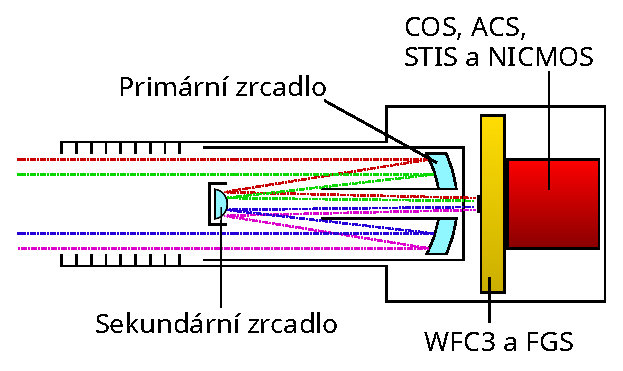
\includegraphics[width=12cm]{hubble-structure.eps}
		\caption{Boční pohled na strukturu optického systému}
		\label{hubble-structure}
	\end{center}
\end{figure}

Klíčovými prvky jsou pochopitelně dvě zrcadla. Větší, primární, zrcadlo má průměr \SI{2.4}{\meter} a poloměr zakřivení \SI{11.04}{\meter}. Sekundární zrcadlo má průměr \SI{0.31}{\meter} a poloměr zakřivení \SI{-1.36}{\meter}.

Sekundární zrcadlo je pohyblivé, aby bylo možné teleskop zaostřit.

Aby do snímacích zařízení nevstupovalo nežádoucí záření, tak je objektiv teleskopu vybaven žebrováním, které toto záření zastaví.

\section{Vesmírný teleskop Jamese Webba}

Druhým teleskopem, který v~tomto projektu představíme, je vesmírný teleskop Jamese Webba. Vesmírný teleskop Jamese Webba (anglicky James Webb Space Telescope, dále v textu jen JWST) je plánovaná vesmírná observatoř, která by měla být vypuštěna v~říjnu 2018. JWST by měl nahradit dosluhující Hubbleův teleskop. V jednotlivých podkapitolách budeme postupně rozebírat jeho zvláštnosti a~parametry. V první řadě se ale zaměříme na jeho historii a~pojmenování.

\subsection{Představení teleskopu} 
JWST je plánovaná velká vesmírná observatoř optimalizovaná pro příjem infračerveného vlnového záření, pomocí kterého budou doplněny a~prohloubeny objevy, které byly uskutečněny Hubbleovým teleskopem.
Díky větší vlnové délce bude JWST schopen pozorovat formování prvních galaxií při utváření vesmíru a dále bude schopen pozorovat formování galaxií, které jsou ukryté za mračny vesmírného prachu.

Původní název JSWT byl Vesmírný teleskop nové generace (anglicky Next Generation Space Telescope, zkráceně NGST). Přívlastek "nové generace" získal proto, že JWST bude stavět a pokračovat ve vědním průzku\-mu, který započal Hubbleův vesmírný teleskop. Objevy, které byly učiněny Hubbleovým teleskopem, ale i ostatními teleskopy, zapříčinily revoluci v astronomii a vyvstaly nové otázky, na jejichž zodpovězení bylo zapotřebí nových, odlišných a výkonnějších teleskopů. 
JWST je také teleskopem nové generace i~po stránce technologické a~to díky použití nových technologií jako například odlehčeného, rozvinovacího primárního zrcadla, které bude určovat technologický směr pro budoucí mise.
Vesmírný teleskop nové generace byl 10. září 2002 přejmenován na Vesmírný teleskop Jamese Webba na počest Jamese E. Webba \cite{nasaFAQ}.
 
\subsubsection{James Edwin Webb}
\begin{wrapfigure}{l}{0cm}
\includegraphics[width=3cm]{webb.eps}
\end{wrapfigure}
James Edwin Webb (1906-1992) byl druhým ředitelem vesmírné agentury NASA. Na pozici ředitele agentury působil od 14. ledna 1961 do 7. října 1968. Během své kariéry se proslavil tím, že byl vedoucím programu Apollo a série misí zaměřených na prozkoumávání měsíčního povrchu, obzvláště mísí, které se zabývaly přistáním prvního člověka na Měsíci. 
Dále inicioval vznik intenzivního vesmírného programu, díky němuž během jeho funkčního období vypravil více než 75 letů a to včetně americké první meziplanetární sondy. Na jeho počest se Vesmírný teleskop nové generace přejmenoval na Vesmírný teleskop Jamese Webba.
\\

\subsection{Poslání a popis teleskopu}
Hlavní mise, kterou by měl JWST po svém vypuštění plnit, se skládá ze čtyř částí.  První částí je hledání světla z prvních hvězd a galaxií, které byly ve vesmíru formovány po Velkém třesku. Druhou částí mise je studování formování a vývoje galaxií. Třetí částí je pochopení formování hvězd a planetárních systémů a poslední částí je studování planetárních systémů a počátku života. \cite{wikipediaWebbEn}. V následujících podkapitolách si představíme, z čeho se JWST skládá, jak je ovládán a kde by se měl po vypuštění pohybovat.

\subsubsection{Zrcadla a optický systém}
Teleskop se skládá z velkého primárního a malého sekundárního a terciálního zrcadla, tepelného štítu a věde\-ckých přístrojů, které jsou popsány níže. Jak již bylo napsáno, JWST bude pracovat v infračerveném spektru, což mu umožní proniknout vesmírným prachem a sledovat velmi vzdálené objekty s nízkou povrchovou teplotou.

Primární zrcadlo JWST má průměr 6.5 metrů a ohniskovou vzdálenost 131.4 metru. Je příliš velké na to, aby bylo dopraveno do vesmíru ve finální podobě, proto se skládá z 18 šestiúhelníkových segmentů vyrobených z berylia. Tím konstruktéři získali celkovou plochu primárního zrcadla 25 m$^2$. Vše je vymyšleno tak, aby se celý teleskop vešel do hlavice nosné rakety.

Každý z šestiúhelníkových dílů primárního zrcadla má v průměru jen něco málo přes 1.3 metru a váží pouhých 40 kg. Tyto díly jsou již vyrobeny a byly dopraveny do Goddardova kosmického střediska, kde se podrobují testům a montují na nosnou konstrukci teleskopu.

Segmenty nejsou jen pouhými zrcadly, ale spíše komplexním souborem technologií, které jim umožňují pracovat jako jeden celek. Zrcadla jsou tvořena zlatem potaženým reflexím beryliovým podkladem, který je ukotvený na delta rám a je schopen pomocí servopohonů změnit pozici a zakřivení vlastního zrcadla. Materiál musel být volen tak, aby byl co nejlehčí a zároveň schopen pracovat při teplotách pod -240 $^\circ$C. Zrcadla přitom musí ustát otřesy a přetížení při startu nosné rakety. Na oběžné dráze se po nich pro změnu požaduje, aby nastavené prvky v neměnné pozici setrvaly ve stabilní poloze až po dobu dvou týdnů. Všechny segmenty jsou rozděleny do tří skupin po šesti zrcadlech, kde každá skupina má lehce odlišnou odrazivou přesnost (viz. obrázek \ref{segmenty}). 

\begin{figure}[h]
\begin{center}
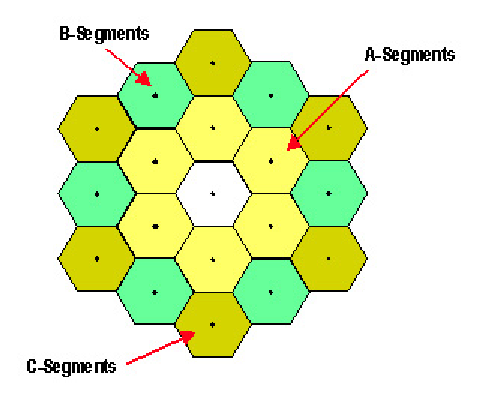
\includegraphics[width=8cm]{webbSegmenty.eps}
\caption{Rozmístění jednotlivých segmentů s různou přesností odrazu na primárním zrcadle}
\label{segmenty}
\end{center}
\end{figure}

\paragraph{Beryliový podklad zrcadla}
Berylium vědci vybrali proto, že je dostatečně tuhé a při tom lehké, ale hlavně, že při změnách teplot chová stabilně a předvídatelně. Konstrukce z tohoto kovu je 5 cm silná s dokonale vybroušenou reflexní plochou. Zadní strana zrcadla má z důvodu odlehčení podobu včelí plástve, jen s tím rozdílem, že podstava je trojúhelníková a ne šestiúhelníková.
Reflexní povrch má přípustnou odchylkou pouhých 20 nanometrů (tj. 20 miliardtin metru). Na něj je nanesena tenká vrstvička zlata, které maximalizuje schopnost odrážet infračervené světlo. 

\paragraph{Beryliové patice}
Na opačné straně od leštěného povrchu jsou upevněny tři trojúhelníkové beryliové patice, pro ukotvení zrcadla k natáčecím servopohonům. Každá patice je asi 30 cm široká a 60 cm dlouhá a rozkládá síly působící v hmotě zrcadla na základní strukturu dbající na stabilitu systému.

\paragraph{Kotvící delta rám}
Beryliové patice jsou osazeny do rámu, který je rovněž z berylia. Rám je hlavní vymezovací strukturou pro každý z 18 primárních segmentů zrcadla. Primární segmenty jsou 75 cm široké a mají tvar písmene delta. Beryliový rám propojuje jednotlivá zrcadla s podkladem, paticemi a servopohony.

\paragraph{Ochranný štít}
JWST bude vybaven speciálním pětivrstvým slunečním štítem, který bude ochraňovat teleskop před slunečním zářením. Díky tomuto štítu bude možno teleskop ochladit na teplotu okolo 50 Kelvina (přibližně -234 $^\circ$C) díky pasivnímu vyzařování tepla do vesmíru. Strana štítu natočená ke Slunci bude zachycovat tepelné záření. Teplota na této straně štítu by se měla pohybovat okolo 85 $^\circ$C a budou zde umístěny komunikační systémy a solární panely. Štít bude mít ve výsledku velikost přibližně tenisového kurtu.

\paragraph{Optická soustava a pozorovací technika}
JWST využívá k pozování tří-zrcadlového anastigmatu - dalekohledu postaveném se třemi zakřivenými zrcadly, které umožní minimalizovat tři hlavní aberace\footnote{odchylky}: sférickou, komu\footnote{projevuje se "kometovým ocasem" u pozorovaných objektů} a astigmatismus\footnote{zaostření pozorovaného objektu}. Tohoto se používá především k tomu, aby bylo možné pozorovat objekty v mnohem větším zorném úhlu, než by umožňovaly teleskopy se dvěma či jednou zakřivenou plochou \cite{wikipediaAnastigmat}.

Paprsky z primárního zrcadla jsou směřovány do sekundárního, které je umístěno před primárním zrcadlem a odtud jsou směřovány do terciálního "zrcadla", které je umístěno přímo uprostřed primárního zrcadla (viz. obrázky \ref{paprskyWebb} a \ref{paprskyWebb2}).

\begin{figure}[h]
\begin{center}
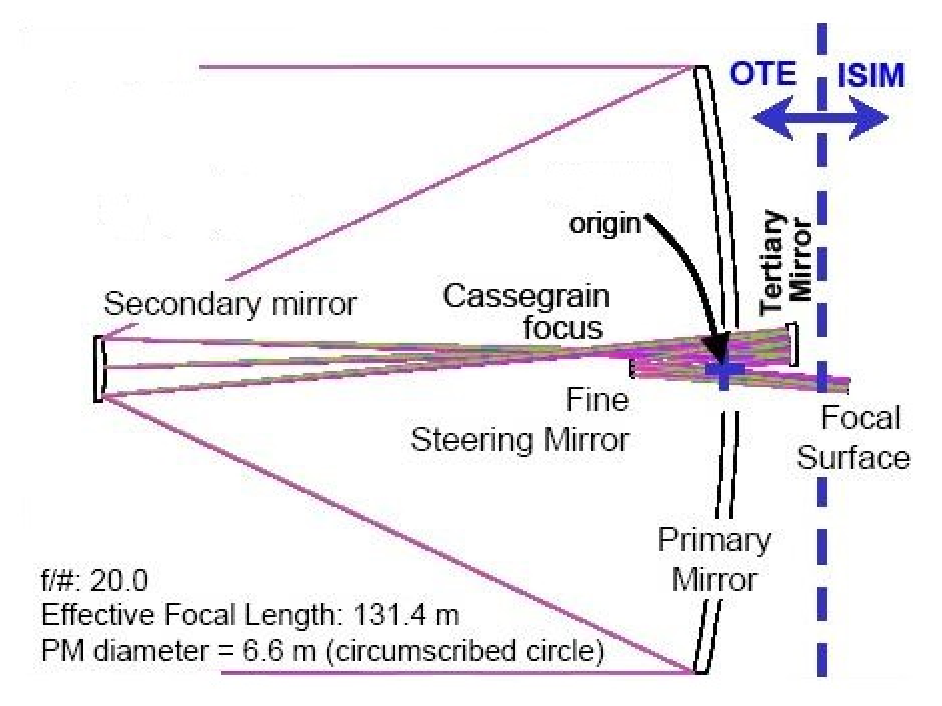
\includegraphics[width=8cm]{webbPaprsky.eps}
\caption{Ukázka způsobu přijímání infračervených paprsků}
\label{paprskyWebb}
\end{center}
\end{figure}


\begin{figure}[h]
\begin{center}
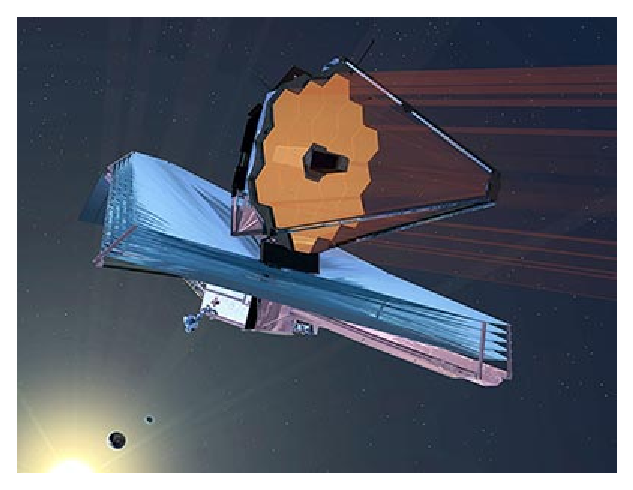
\includegraphics[width=8cm]{webbPaprsky2.eps}
\caption{Ukázka přepokládaného umístění teleskopu ve vesmíru a způsob přijímání infračerveného záření, které je naznačeno červenými paprsky}
\label{paprskyWebb2}
\end{center}
\end{figure}

Takto přijaté paprsky jsou následně zpracovávány několika přístroji, kterými bude JWST disponovat. Tyto přístroje budou umístěny přímo za primárním zrcadlem JWST. V informacích o JSWT jsou tyto přístroje souhrnně pojmenovány jako integrovaný modul vědeckých přístrojů (zkráceně ISIM). 

Near InfraRed Camera (NIRCam) - kamera vybavená přístrojem, který umožní odstínit světlo hvězdy a studovat tak její okolí (například planety). Zaměří se na studium starých hvězd ve vzdálených galaxiích i ledová tělesa daleko za dráhou Neptunu.

Near InfraRed Spectrograph (NIRSpec) - sektrograf určený pro studium složení, teploty a hmotnosti vzdálených nebeských objektů.

Mid-InfraRed Instrument (MIRI) - kamera a spektrograf v jednom. Zaměří se na studium nejstarších galaxií a hvězd stejně jako slabých komet.

Fine Guidance Sensor / Near InfraRed Imager and Slitless Spectrograph (FGS/NIRISS) - další spektrograf jehož úkolem je zkoumat složení planet u cizích hvězd \cite{abcko}.

\subsubsection{Ovládání segmentů primárního zrcadla}
Tvarování povrchu a vyrovnávání povrchu primárního zrcadla zajišťují servopohony. Starají se o všech 18 primárních segmentů, výsledkem je ostrý obraz i při dlouhé expozici a měnících se teplotních podmínkách.


Každý z hlavních segmentů zrcadla má šest pohonných jednotek, jen tak šlo docílit aby výsledné monolitické zrcadlo bylo co nejdokonalejší. Specialitou je pak servopohon připojený přímo do středu zadní části zrcadla prostřednictvím dlouhých, tenkých beryliových podpěr vedoucích až k okrajům zrcadla. Ty zajišťují, aby každé ze zrcadel mělo stejnou ohniskovou vzdálenost.


Servopohony jsou jednou z mnoha součástí vytvořených speciálně pro JWST. Jejich úkolem je provádět změny v rozměrech nanometrů. Právě tím bude teleskop dosahovat své optické dokonalosti. Pro lepší představu, jak je zařízení přesné, si můžeme vzít do ruky kancelářský papír. Ten má  tloušťku okolo  100 000 nm. Změny odrazové plochy zrcadla se upravují v měřítku  1 / 100 000 tloušťky běžného papíru. A nejen to. Pohony musí pracovat spolehlivě i když teplota klesne na hodnotu několika desítek stupňů nad absolutní nulu.

Po vypuštění JWST budeme muset na první snímky nějakou dobu počkat. Nejprve se bude  stabilizovat na provozní teplotu. Pak technici začnou pomocí příkazů ze Země testovat funkci servopohonů. Bude to trvat zhruba dva měsíce a teprve pak začne být JWST uváděn do provozu a začne s vědeckým pozorováním. Jemné dolaďování zrcadel budou vědci provádět jednou za 10 až 14 dnů. JWST bude první vesmírnou observatoří používající aktivně řízené segmentové primární zrcadlo.

\paragraph{Kotvení zrcadla k hlavní konstrukci}
Pro připojení jednotlivých zrcadel k hlavní nosné konstrukci teleskopu jsou použity pružné tvarovky – Flextures. Fungují jako pružiny. Flextures dovolují rozpínání a smršťování celé soustavy zrcadel, ke kterému dochází změnami teplot  už v rámci předletových kontrol zde na Zemi. Cílem je otestovat tvarovou stabilitu JWST před jeho velkým ochlazením, ke kterému dojde ve vesmíru a kde provozní teplota bude okolo 50 K (-223 $^\circ$C) \cite{osel}.

\subsubsection{Umístění teleskopu}
Narozdíl od svého předchůdce (Hubbleův teleskop) se JWST nebude pohybovat na nízké oběžné dráze, ale bude umístěn v Lagrangeově bodě L2 soustavy Země - Slunce, tedy asi 1,5 mil. km od Země, na opačné straně než Slunce. Teleskop bude obíhat po eliptické dráze s poloměrem přibližně 800 000 km v okolí bodu L2. Tuto dráhu by měl být schopen zvládnout za půl roku.

Lagrangeův bod je v nebeské mechanice takový bod v soustavě dvou těles \begin{math}m_1\end{math} a \begin{math}m_2\end{math} rotujících kolem společného těžiště, v němž se vyrovnávají gravitační a odstředivé síly soustavy tak, že malé těleso umístěné do tohoto bodu nemění vůči soustavě svou polohu. Všechny Lagrangeovy body se nachází v rovině rotace těchto těles a je jich celkem pět. Označují se L1 až L5. Vlastnosti Lagrangeových bodů popsal v roce 1772 francouzský matematik a fyzik Joseph Louis Lagrange \cite{lagrange}.
\begin{figure}[h]
\begin{center}
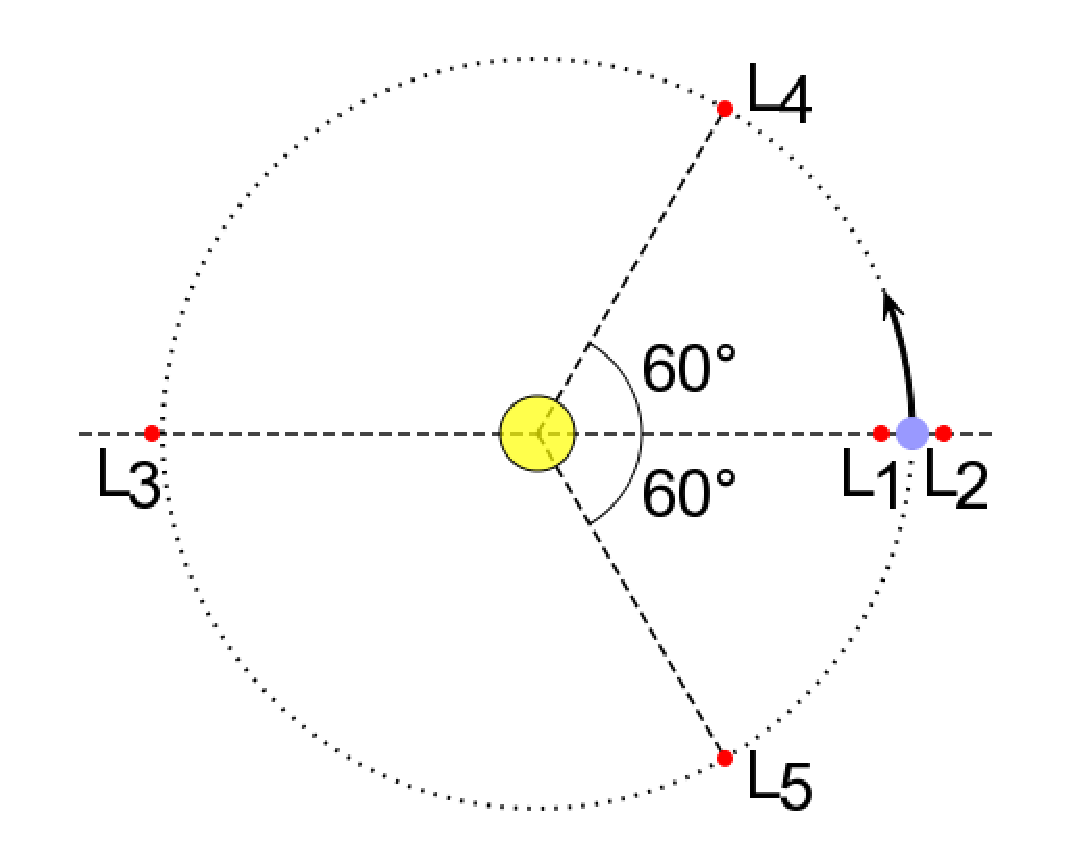
\includegraphics[width=8cm]{lagrange.eps}
\caption{Lagrangeovy body soustavy s velmi těžkým centrálním tělesem (jako je Slunce v soustavě Slunce - Země)}
\end{center}
\end{figure}

Servisní lety současnými běžnými pilotovanými prostředky k tomuto teleskopu jsou díky jeho vzdálenosti od Země prakticky vyloučeny. JWST bude na místo určení vynesen raketou Ariane 5.

Od roku 2005 byl velký model JWST byl postupně představen na několika místech na světě. V USA byl vystaven v Seattlu ve státě Washington, v Colorado Springs ve státě Colorado, v Greenbeltu ve státě Maryland, v Rochesteru a na Manhattanu ve státě New York a v Orlandu na Floridě. Dále byl představen v Paříži, Dublinu, Montrealu, Hatfieldu a Mnichově. Model byl vybudován hlavním partnerem tohoto projektu, firmou North Grumman Aerospace Systems.

V roce 2007 byl model teleskopu v životní velikosti vystaven ve Washingtonu D.C., aby si díky němu lidé lépe představili rozměry a komplexitu satelitu. Tento model byl z důvodl působení gravitace a počasí vyroben z hliníku a oceli. Model má rozměry 24x12x12 metrů a je těžký 5.5 tuny \cite{wikipediaWebbEn}.

\begin{figure}[h]
\begin{center}
\includegraphics[width=8cm]{webbModel.eps}
\caption{Vystavený model JWST}
\end{center}
\end{figure}

\section{Srovnání Hubbleova teleskopu s Teleskopem Jamese Webba}
Velmi krátce zde na názorných obrázcích představíme rozdíly mezi Hubbleovým teleskopem a Teleskopem Jamese Webba.

\begin{figure}[h]
\begin{center}
\includegraphics[width=8cm]{mirrors.eps}
\caption{Názorné srovnání velikosti primárního zrcadla obou teleskopů}
\end{center}
\end{figure}

\begin{figure}[h]
\begin{center}
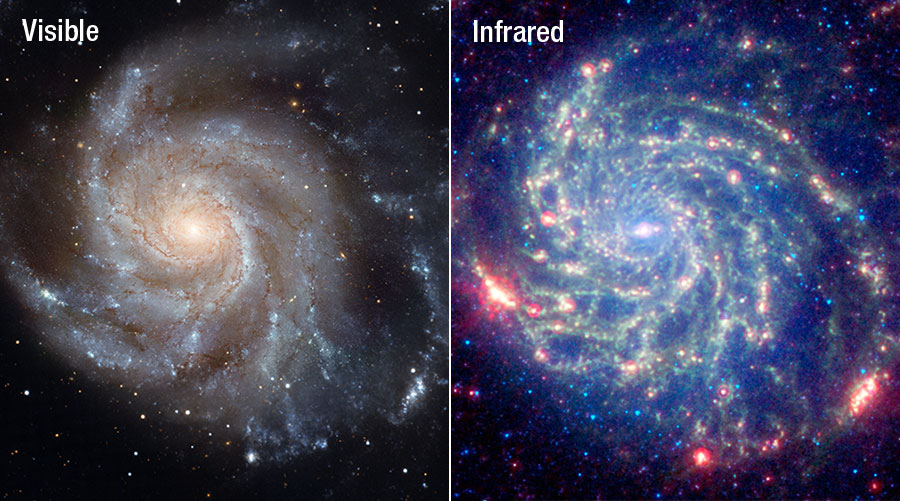
\includegraphics[width=8cm]{compare.jpg}
\caption{Srovnání obrazu z Hubbleova teleskopu (viditelné spektrum) a odhadovaného obrazu z JWST (infračervené spektrum)}
\end{center}
\end{figure}

\section{Závěr}
V této práci jsme představili dva teleskopy. Aktuálně využívaný Hubbleův teleskop a jeho nástupce, který je právě budován, Vesmírný teleskop Jamese Webba. Snažili jsme se u každého teleskopu popsat jeho historii, strukturu a optický systém. V poslední kapitole jsme uvedli viditelné rozdíly mezi oběma teleskopy.
\newpage

\bibliographystyle{czechiso}
\def\refname{Použitá literatura}
\bibliography{dokumentace}

\end{document}
